% ============================================================================
\section{Common-Mode Voltage Effects}
\label{sec:common_mode}
% ============================================================================

In any converter-fed ac machine, the non-zero average of the three
phase-leg pole voltages produced by PWM switching gives rise to a
common-mode voltage (CMV) that excites parasitic capacitive paths
between winding, frame, shaft, and bearings. This mechanism is well
characterized for a converter with a single machine port whose voltage
scaling is produced internally, such as the flying-capacitor
multilevel converter, for which an analytical CM-EMI model referenced
to one dc-link potential exists \cite{Giardine2025FCMLEMI}. SPB does
not fit this picture: because its $N$ cells are connected in series on
the dc side (Section~\ref{sec:operating_principle}) while each feeds
an electrically separate winding group, cell $k$'s local dc rails are
displaced from the overall dc-bus reference by an amount that depends
on its position in the stack.

\subsection{Series-Stack Origin of Common-Mode Excitation}

Taking cell 1's negative dc rail as the reference, with cell $k$'s
negative rail coinciding with cell $(k-1)$'s positive rail, the
absolute offset of cell $k$ is

\begin{equation}
V_{-,k}=\sum_{j=1}^{k-1}V_{\mathrm{dc},j}
\approx(k-1)\frac{V_{\mathrm{dc}}}{N},
\label{eq:spb_cm_offset}
\end{equation}

using the voltage-partitioning relation \eqref{eq:spb_voltage_sum}. The
common-mode potential seen by winding group $k$ is then

\begin{equation}
v_{\mathrm{cm},k}^{\mathrm{abs}}(t)=
V_{-,k}+\frac{1}{3}\left(v_{aN_k}+v_{bN_k}+v_{cN_k}\right),
\label{eq:spb_cm_local}
\end{equation}

where $v_{aN_k},v_{bN_k},v_{cN_k}$ are cell $k$'s pole voltages
referenced to its own negative rail $N_k$. The second term is the
conventional switching-induced CMV already addressed by zero-sequence
injection and vector-redundancy modulation
(Section~\ref{sec:modulation}); the first term, $V_{-,k}$, is specific
to SPB, set by the cell's stack position and by the instantaneous
voltage-sharing state (Section~\ref{sec:dclink_balancing}), not by
modulation alone.

Fig.~\ref{fig:spb_cm_stack} illustrates the resulting structure:
increasing absolute potential offset with stack position, together
with representative CM current paths coupling each winding group to
the shared frame and chassis ground through parasitic capacitance.
Because the cells and their winding groups are physically close
together in the integrated implementations of
Section~\ref{sec:machine_requirements}, these paths are short and the
coupling between cells is direct rather than mediated by long cabling.
Physically integrated motor-drive assemblies show that common-mode
current can resonate through exactly this kind of parasitic loop, and
that the resonance is not adequately predicted by a single-source CM
model \cite{Zhong2025CMResonance,Chen2020EMCIntegrated} -- extending
such modeling to a multi-port structure with $N$ distinct dc offsets
is, to the authors' knowledge, not yet available for SPB specifically.

\begin{figure}[!t]
\centering
\begin{tikzpicture}[font=\scriptsize,>=latex,node distance=5mm]
\tikzstyle{cell}=[draw=blue!65!black,rounded corners,minimum width=17mm,
  minimum height=9mm,align=center,fill=blue!8,font=\tiny]
\tikzstyle{wind}=[draw=orange!75!black,rounded corners,minimum width=19mm,
  minimum height=8mm,align=center,fill=orange!12,font=\tiny]
\tikzstyle{gndbox}=[draw=teal!60!black,rounded corners,minimum width=24mm,
  minimum height=7mm,align=center,fill=teal!8,font=\tiny]

\node[cell] (cN) {\textbf{Cell $N$}\\ offset $V_{-,N}$};
\node[font=\scriptsize,below=3mm of cN] (dots) {$\vdots$};
\node[cell,below=3mm of dots] (c2) {\textbf{Cell 2}\\ offset $V_{-,2}$};
\node[cell,below=5mm of c2] (c1) {\textbf{Cell 1}\\ offset $V_{-,1}{=}0$};

\node[wind,right=13mm of cN] (wN) {Winding group $N$};
\node[wind,right=13mm of c2] (w2) {Winding group 2};
\node[wind,right=13mm of c1] (w1) {Winding group 1};

\draw[->] (cN.east) -- (wN.west);
\draw[->] (c2.east) -- (w2.west);
\draw[->] (c1.east) -- (w1.west);

\coordinate (topdc) at ([yshift=4mm]cN.north);
\draw[thick] (topdc) -- (cN.north);
\node[font=\tiny,left] at (topdc) {$+$};
\draw[thick] (cN.south) -- (dots.north);
\draw[thick] (dots.south) -- (c2.north);
\draw[thick] (c2.south) -- (c1.north);
\coordinate (botdc) at ([yshift=-4mm]c1.south);
\draw[thick] (c1.south) -- (botdc);
\node[font=\tiny,left] at (botdc) {$-$};

\node[gndbox,below=11mm of w1,xshift=10mm] (gnd)
  {Frame / chassis\\ ground reference};

\coordinate (busN) at ([xshift=10mm]wN.east);
\coordinate (bus2) at ([xshift=10mm]w2.east);
\coordinate (bus1) at ([xshift=10mm]w1.east);

\draw[teal!60!black,dashed] (wN.east) -- (busN);
\draw[teal!60!black,dashed] (w2.east) -- (bus2);
\draw[teal!60!black,dashed] (w1.east) -- (bus1);
\draw[teal!60!black,dashed] (busN) -- (bus1);
\draw[teal!60!black,dashed,->] (bus1) -- (gnd.north);
\node[font=\tiny,teal!60!black,align=center,rotate=90] at ([xshift=4mm]bus2)
  {CM current paths\\(parasitic coupling)};
\end{tikzpicture}
\caption{Simplified SPB series-stack structure: absolute potential
offset per cell \eqref{eq:spb_cm_offset} and representative CM current
paths (dashed) to the shared frame/chassis ground through parasitic
capacitance.}
\label{fig:spb_cm_stack}
\end{figure}

\subsection{Carrier Synchronization for CMV Cancellation}

Beyond the stack-offset mechanism above, synchronizing each cell's PWM
waveform relative to the others is a way to actively cancel the
switching-induced component of CMV. We illustrate the principle for
the $N=2$ case, where the cancellation condition has a simple closed
form; the same synchronization idea extends to larger stacks built
from matched cell pairs, though a general $N$-cell synchronization law
has not yet been derived for SPB.

If cell 2 is driven with the logical inverse of cell 1's gate
commands, and cell 2's winding set is wired with reversed winding
sense so that both cells still generate torque in the same direction,
the two cells' individually switched CMVs become approximately equal
and opposite, $v_{\mathrm{cm},1}(t)\approx-v_{\mathrm{cm},2}(t)$, and
the total CMV seen by the machine,
\begin{equation}
v_{\mathrm{cm,tot}}(t)=\frac{v_{\mathrm{cm},1}(t)+v_{\mathrm{cm},2}(t)}{2},
\label{eq:spb_cm_cancellation}
\end{equation}
cancels toward zero instead of adding constructively. This
balanced-cancellation principle was first demonstrated for a
dual-winding-set machine driven by a balanced inverter pair on a
single, non-series-stacked machine \cite{Han2018CMCancellation}, and
was later applied to a genuine two-cell series-stacked (2L-SSC) SPB
inverter \cite{Rohner2024GaN}; as with interleaved GaN IMMDs, the
achievable reduction is ultimately limited by layout parasitics and
local dc-link capacitor design \cite{Wang2015GaNIMMD}.

This cancellation assumes perfectly matched, simultaneous switching
transitions between the two cells: a propagation-delay mismatch (e.g.,
from PCB layout or driver differences) reintroduces a residual CM
spike, of duration equal to the delay, at every misaligned transition,
and unequal power sharing during dc-link balancing similarly degrades
the cancellation, both shown quantitatively in
\cite{Rohner2024GaN,Han2018CMCancellation}. The mechanism is specific
to $N=2$, or to a stack of matched cell pairs, so it should be read as
a valuable special-case mitigation rather than a general solution to
the stack-offset problem above. Fig.~\ref{fig:spb_cm_cancellation}
simulates this cancellation directly from switching-function
waveforms, including its effect on the resulting bearing/ground
current.

\begin{figure}[!t]
\centering
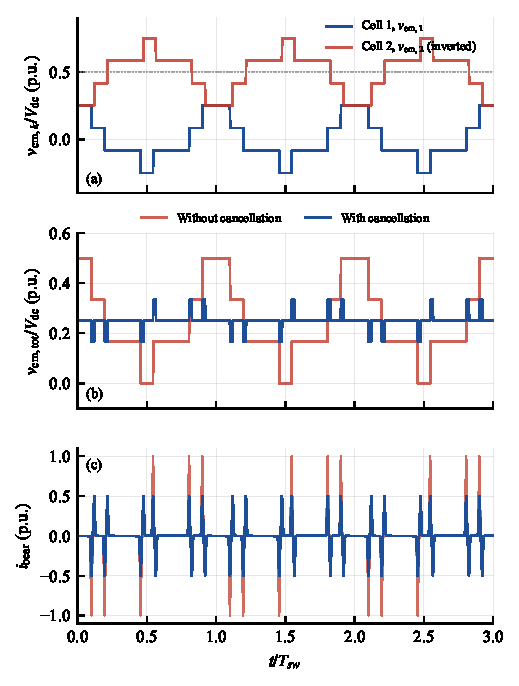
\includegraphics[width=\columnwidth]{Figures/fig_cm_cancellation.pdf}
\caption{Switching-function simulation of $N=2$ SPB common-mode
cancellation ($M=0.85$, $\cos\varphi\approx0.94$), all quantities in
per unit, with cell~2 driven by the logically inverted gate commands of
cell~1 plus a propagation delay $t_d=0.02\,T_{sw}$. (a)~Each cell's
absolute CM voltage $v_{\mathrm{cm},k}^{\mathrm{abs}}$, combining the
stack offset $V_{-,k}$~\eqref{eq:spb_cm_offset} with its local
switching term. (b)~Total CM voltage
$v_{\mathrm{cm,tot}}(t)$~\eqref{eq:spb_cm_cancellation}: cancellation
removes the switching ripple, leaving only delay-induced residual
spikes on the same stack-offset average. (c)~Resulting bearing/ground
current $i_{\mathrm{bear}}=C\,dv_{\mathrm{cm,tot}}/dt$, normalized to
the without-cancellation peak. Computed simulation result, not
measured hardware data.}
\label{fig:spb_cm_cancellation}
\end{figure}

\subsection{Physical Consequences and Mitigation}

CMV-driven bearing current is a documented failure mechanism in
inverter-fed machines generally, arising from capacitive coupling
through the air gap and discharge events once the bearing lubricant
film breaks down \cite{Lee2025BearingCurrent}, and can be identified
with dedicated non-intrusive current-measurement techniques
\cite{Li2025BearingMeasurement}. In SPB, this mechanism acts at each of
the $N$ winding groups individually; because
\eqref{eq:spb_cm_offset}--\eqref{eq:spb_cm_local} gives each group a
different absolute CM reference, the resulting bearing- and
shaft-voltage stress is not necessarily uniform across the stack, and
whether it is dominated by the highest-offset cell, by all cells
combined, or by resonant interaction between cells remains open.
Shaft-voltage cancellation circuits developed for conventional drives
\cite{Xie2026ShaftCM} are a plausible mitigation candidate but have not
been demonstrated for a series-stacked, multi-port machine.

The same switching events also produce fast $dv/dt$ transitions at the
winding terminals, stressing turn-to-turn and phase-to-frame
insulation independently of the CM current path. WBG devices, already
motivated for SPB by their favorable scaling at reduced blocking
voltage (Section~\ref{sec:semiconductor_scaling}), shorten rise time
and increase overshoot, and have been shown to accelerate insulation
aging and partial-discharge activity in hairpin and other
traction-machine windings \cite{KholghKhiz2025HairpinWBG,
Gulec2025PDImpulse,Seri2025ATFPDIV}; diagnostic methods exist to assess
the resulting insulation condition \cite{Kim2025HairpinFRA}, within the
broader set of insulation technologies for transport-electrification
machines \cite{Martinez2025TransportInsulation}. In SPB, this stress is
superimposed on the stack-position-dependent offset of
\eqref{eq:spb_cm_offset}, so insulation coordination must account for
both the local switching transition and the cell's absolute stack
position, consistent with the challenge identified qualitatively in
Section~\ref{sec:machine_requirements}.

Mitigation therefore has to act at more than one level. Active EMI
filtering can attenuate common-mode current at the converter terminals
without relying on machine or bearing hardware
\cite{Ihsan2025ActiveEMI}, and cancellation circuits can target shaft
voltage directly \cite{Xie2026ShaftCM}. At the modulation level,
Section~\ref{sec:modulation} showed that zero-sequence injection and
redundant-vector selection reduce CMV excitation
\cite{Sun2025CMVMPC,Zheng2025MultiObjectivePWM}, but the carrier-phase
displacement used there to interleave switching harmonics for ripple
reduction, \eqref{eq:carrier_phase}, is chosen to cancel a selected
ripple harmonic and is not simultaneously optimized for common-mode
excitation. Because SPB's CM problem additionally depends on the fixed
stack offset $V_{-,k}$, which carrier phasing cannot change, an
interleaving choice that minimizes dc-link or stator ripple need not
minimize aggregate common-mode excitation, and vice versa -- a genuine
SPB-specific design tension that future studies should address by
extending the multi-objective modulation problem of
Section~\ref{sec:modulation} to common-mode and insulation-stress
metrics evaluated across the full stack.
